\documentclass[class=report, crop=false, 12pt,a4paper]{standalone}
\usepackage{enumitem}
\usepackage{multicol}
\usepackage{etoolbox}
\AtBeginEnvironment{quote}{\singlespacing\small}
\usepackage{setspace}
\onehalfspacing
\usepackage{graphicx}
\usepackage{siunitx}
\usepackage{amsmath}
\sisetup{detect-all}
\begin{document}
\section{Dimensionless Numbers}
\subsection{Notation}
We denote a dimension by using a capital letter in square brackets. Here are some common dimensions.
\begin{itemize}[noitemsep]
  \item {[M]} - mass (unit: kilogram).
  \item {[T]} - time (unit: second).
  \item {[L]} - length (unit: metre).
  \item {[\(\Theta\)]} - temperature (unit: kelvin).
\end{itemize}
Thus, we can derive that the dimensions of acceleration (which has units \si{\meter\per\second\squared}) [L][T]\(^{-2}\). Some dimensions of common measurements are shown below:
\begin{itemize}[noitemsep]
  \item Force - [M][L][T]\(^{-2}\).
  \item Energy - [M][L]\(^2\)[T]\(^{-2}\).
\end{itemize}
We use dimensional analysis to check derivations. The dimensions of both sides of any equation must match. Physical constants also often have units associated with them - these must also be considered. Some variables are dimensionless such as the Reynolds number.
\begin{gather} 
  Re = \frac{\rho l u}{\mu}\\
  [Re] = \frac{[M][L]^{-3}\cdot [L] \cdot [L][T]^{-1}}{[L][M][T]^{-2}\cdot [T][L]^{-2}} = \frac{[M][L]^{-1}[T]^{-1}}{[M][L]^{-1}[T]^{-1}} 
\end{gather}
Hence, we can see that the Reynolds number is a dimensionless quantity as all the dimensions cancel.
\subsection{Example}
We can use dimensional analysis to derive basic forms of equations. We want to work out the pressure drop as oil flows though a pipe. Let us consider the parameters this may depend on. 
\begin{itemize}[noitemsep]
  \item Viscosity - [M][L]\(^{-1}\)[T]\(^{-1}\).
  \item Pipe length - [L].
  \item Pipe diameter - [L].
  \item Velocity - [L][T]\(^{-1}\).
  \item Pressure - [M][L]\(^{-1}\)[T]\(^{-2}\).
\end{itemize}
Next we can assume that the pressure is a function of the other four. Some combination of the others must have the same dimension as the quantity we want.
\begin{gather} 
  [M][L]^{-1}[T]^{-2} = ([M][L]^{-1}[T]^{-1})^\alpha \cdot ([L])^\beta \cdot ([L])^\gamma \cdot ([L][T]^{-1})^\delta \\
  [L]: -1 = -\alpha + \beta + \gamma + \delta\\
  [M]: 1 = \alpha \\
  [T]: -2 = -\alpha -\delta \\
  \alpha =1, \ \delta =1, \ \beta + \gamma = -1
\end{gather}
So it must be true that:
\begin{equation} 
  \Delta P = \mu \cdot v \cdot I^{\beta} \cdot D^{\gamma}
\end{equation} 
Where \(\beta + \gamma = -1\)
The actual answer for laminar flow is:
\begin{equation} 
  \Delta P = \frac{2\mu L v}{D^2}
\end{equation}
This sort of analysis is useful for checking on the functional form of relationships, but it won't give you the exact relationship, or the value of any dimensionless constants involved.
\subsection{Similarity}
\begin{itemize}[noitemsep]
  \item Geometrical similarity: fixed ratio of lengths.
  \item Kinematic similarity: fixed ratio of velocities.
  \item Dynamic similarity - fixed ratio of forces.
\end{itemize}
Note on inertia: Inertia is not a force. However, for considering its importance to dynamic similarity, we can use the force needed to slow down a moving object. So we quantify inertia for these purposes as \(ma\), from \(F = ma\). Since the forces on flow change fluid motion, we use this often. 
\subsubsection{Dynamic similarity: viscosity}
Compare the inertia "force" and the viscous force for a fluid:
\begin{equation} 
  \frac{[Inertia \ force]}{[Viscous \ force]} = \frac{\rho L^2 u^2}{\mu u L} = \frac{\rho L u }{\mu} 
\end{equation}
The Reynolds number is something very specific - it allows us to calculate the ratio of inertial and viscous forces in order to check for dynamical similarity.
\begin{itemize}[noitemsep]
  \item Honey: Re \(\approx 1.3 \times 10^{-4}\)
  \item Tea: Re \(\approx 1100 \)
\end{itemize}
Therefore, they are not dynamically similar with respect to viscosity. 
For complete dimensional similarity, we must match the Reynolds number with the Froude number. If the same working fluid is used for the model and the prototype it is not possible to match the Reynolds number and the Froude number except if the model and the prototype have the same length. To achieve complete dynamic similarity between geometrically similar flows, it is necessary to duplicate the values of the independent dimensionless groups; by so doing the value of the dependent parameter is then duplicated. This is important because measured values of drag from model test could be scaled to predict drag for the operating conditions of the prototype. INSERT EXAMPLE MERT
\subsection{Dimensionless groups}
We have identified some dimensionless groups such as Reynolds number and Froude number. There are many more such as:
\begin{itemize}[noitemsep]
  \item Bond number: ratio of gravitational to surface tension forces.
  \item Capillary number: ratio of surface tension to viscous forces.
  \item Euler number: ratio of pressure force to inertial force.
  \item Grashof number: ratio of buoyancy to viscous forces.
  \item Cauchy number: ratio of inertial to elastic forces.
  \item Weber number: ratio of inertial to surface tension forces.
\end{itemize}
\section{Integration over areas}
1D integrations allows you to sum a function with respect to one variable.
\begin{equation}
  I = \int_{x_0}^{x_1} F(x) dx
\end{equation}
Where $x_0$ and $x_1$ are the lower and upper limits respectively. If our function varies with two variables, we have $F(x, \ y)$. In order to integrate this, we need to use double integration.
\begin{equation}
  I = \int \int_x^y F(x, \ y)dxdy
\end{equation}
The product $dxdy$ is the area of a small element on the x-y plane and we may also label it $dA$, where $A$ represents the area.
\begin{figure}
  \centering
  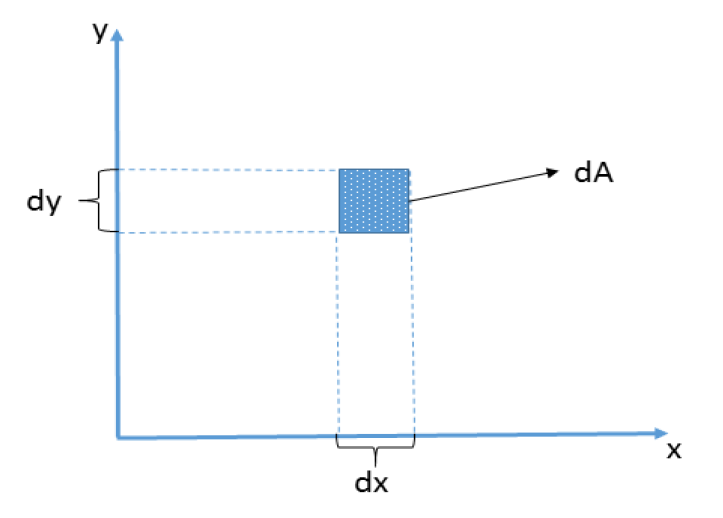
\includegraphics[width = 0.7\textwidth]{../img/doubleintegration}
  \caption{The resulting area $dA$ when utilising double integration.}
\end{figure}
Because $A$ represents the area, you may also see this written like this:
\begin{equation}
  I = \int_A F(x, \ y) dA
\end{equation}
These two notations are equivalent. The subscript $\int_A$ just means an integration over all $A$, just as $\int_x$ means an integration over all x.
In most of the problems you will deal with, the order of the integration is not important – it doesn’t matter whether you integrate over x first or y first.
By convention, the inner one is done first, so 
\begin{equation}
  I = \int \int_x^y F(x, \ y) dxdy
\end{equation}
implies that the integration will be done in the x-direction first, then in the y-direction.

Consider this function
\begin{equation}
  F(x, \ y) = 3x^2 + 2y
\end{equation}
We want to sum this quantity over the x-y plane. For example, $F(x,\ y)$ could represent the volume flow through that element of the plane per unit time. Adding up that quantity for every element of the plane will give us the volume flow through the entire area, per unit time.
\begin{equation}
  I = \int_{Y_0}^{Y_1}(2x^2 + 2y)dxdy
\end{equation}
We carry out the inner integration first, treating y as though it were a constant:
\begin{equation}
  I = \int^{Y_1}_{Y_0}\left(x^3 + 2yx \right)^{X_1}_{X_0} dy = \int_{Y_0}^{Y_1} \left( (X^3_1 +2yX_1) - (X^3_0 + 2yx_0) \right) dy
\end{equation}
Then we integrate this with respect to dy:
\begin{align}
  I &= \int_{Y_0}^{Y_1} \left( (X^3_1 - X^3_0) + 2y(X_1 - X_0) \right) dy = \left( y(X^3_1 - X^3_0) + y^2(X_1 - X_0) \right)^{Y_1}_{Y_0}\\
  I &= (Y_1 - Y_0)(X^3_1 - X^3_0) + (Y^2_1 - Y^2_0)(X_1 - X_0)
\end{align}
This is not always the most efficient way to integrate over an area. We can construct elements dA in whatever shape is most convenient.
\begin{figure}
  \centering
  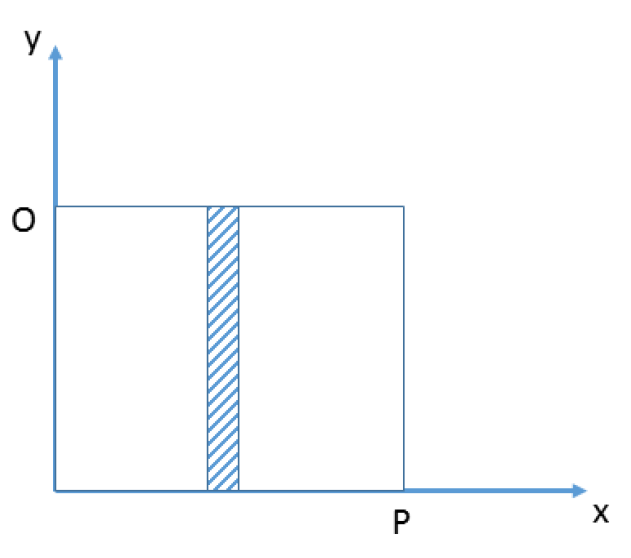
\includegraphics[width = 0.5\textwidth]{../img/areaofrectangle}
  \caption{A rectangle.}
\end{figure}
To find the area of a rectangle, we could integrate over all the elements dA = dxdy.
But because of the symmetry of the problem, we can also choose a strip to integrate over:
\begin{equation}
  I = \int_x O dx
\end{equation}
This means adding up all the strips, each one of area $O dx$.
For a circle, we can split the area into concentric rings:
\begin{figure}
  \centering
  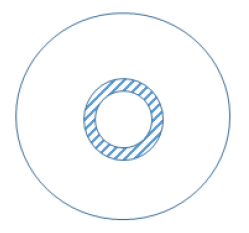
\includegraphics[width = 0.5\textwidth]{../img/areaofcircle}
  \caption{A circle.}
\end{figure}
The area of this ring is $2\pi dr$. To calculate the area of the circle, we can just add up all the rings out to same radius R:
\begin{equation}
  A = \int_0^R (2\pi r)dr = \int_0^R dA = 2\pi \int_0^R (r) dr = 2\pi \left[ \frac{1}{2} r^2 \right]^R_0 = \pi R^2
\end{equation}
Now consider a pipe with a circular cross-section. Water is flowing steadily through the pipe, but it has a different velocity at different radii. Suppose that the velocity is given by:
\begin{equation}
  v(r) = (R-r)^2 = r^2 - 2Rr + R^2
\end{equation}
where $R$ is the radius of the pipe.
Consider a ring of radius r and dr wide. The volume of water passing through this ring per unit time is:
\begin{equation}
  V(r) = v(r)dA
\end{equation}
the velocity (is the distance travelled in 1 second) multiplied by the area of the ring.
We want to find the total volume flowing through the pipe per unit time, so we want to add up the flow through each ring.
\begin{equation}
  Flow = \int_0^R v(r)dA
\end{equation}
We know that $dA = 2\pi r dr$, and we know $v(r)$:
\begin{align}
  F &= \int_0^R ((r^2 - 2Rr + R^2)2\pi r) dr\\
  &= 2\pi \int (r^3 - 2Rr^2 + R^2r) dr\\
  &= 2\pi \left[ \frac{1}{4} r^4 - \frac{2}{3} R r^3 + \frac{1}{2} R^2 r^2 \right]^R_0\\
  &= \frac{\pi R^4}{6}
\end{align}
By choosing dA appropriately, we can integrate quantities over specific areas. You’ll learn to choose the most efficient dA with experience.
\end{document}